\documentclass[aspectratio=169]{beamer}

\usetheme{metropolis}
\usepackage{appendixnumberbeamer}
\usepackage{booktabs}
\usepackage{amsmath,amssymb}
\usepackage{siunitx}
\sisetup{group-separator={,}, group-minimum-digits=4}
\usepackage{tikz}
\usetikzlibrary{arrows.meta,positioning,shapes.geometric}
\usepackage{graphicx}

\definecolor{revenue}{HTML}{2E7D32}
\definecolor{cost}{HTML}{C62828}
\definecolor{accent}{HTML}{1565C0}

\title{Techno-Economic Assessment of\\[4pt] \textbf{Steel Slag} Valorization}
\subtitle{H\textsubscript{2} Production $\cdot$ CO\textsubscript{2} Sequestration $\cdot$ Iron Recovery}
\author{Step Function LLC}
\institute{Separation-Agents Framework}
\date{\today}

\begin{document}

% ═══════════════════════════════════════════════════════════════
\begin{frame}
\titlepage
\end{frame}

% ═══════════════════════════════════════════════════════════════
\begin{frame}{Outline}
\tableofcontents
\end{frame}

% ═══════════════════════════════════════════════════════════════
\section{Background}
% ═══════════════════════════════════════════════════════════════

\begin{frame}{Opportunity: BOF Steel Slag}
\begin{columns}
\column{0.55\textwidth}
\begin{itemize}
    \item \textbf{250+ Mt/yr} slag produced globally
    \item Mostly landfilled — environmental liability
    \item Rich in CaO, FeO/Fe\textsubscript{2}O\textsubscript{3}, MgO, SiO\textsubscript{2}
\end{itemize}
\vspace{8pt}
\textbf{Three valorization pathways:}
\begin{enumerate}
    \item Green H\textsubscript{2} (serpentinization)
    \item CO\textsubscript{2} sequestration (carbonation)
    \item Iron concentrate (magnetic sep.)
\end{enumerate}

\column{0.42\textwidth}
\begin{table}
\centering
\small
\begin{tabular}{@{}lc@{}}
\toprule
\textbf{Component} & \textbf{wt\%} \\
\midrule
CaO & 40 \\
Fe\textsubscript{2}O\textsubscript{3} & 15 \\
FeO & 15 \\
SiO\textsubscript{2} & 20 \\
MgO & 10 \\
\bottomrule
\end{tabular}
\caption*{BOF slag composition}
\end{table}
\end{columns}
\end{frame}

% ═══════════════════════════════════════════════════════════════
\section{Process Design}
% ═══════════════════════════════════════════════════════════════

\begin{frame}{Process Flow Diagram}
\begin{center}
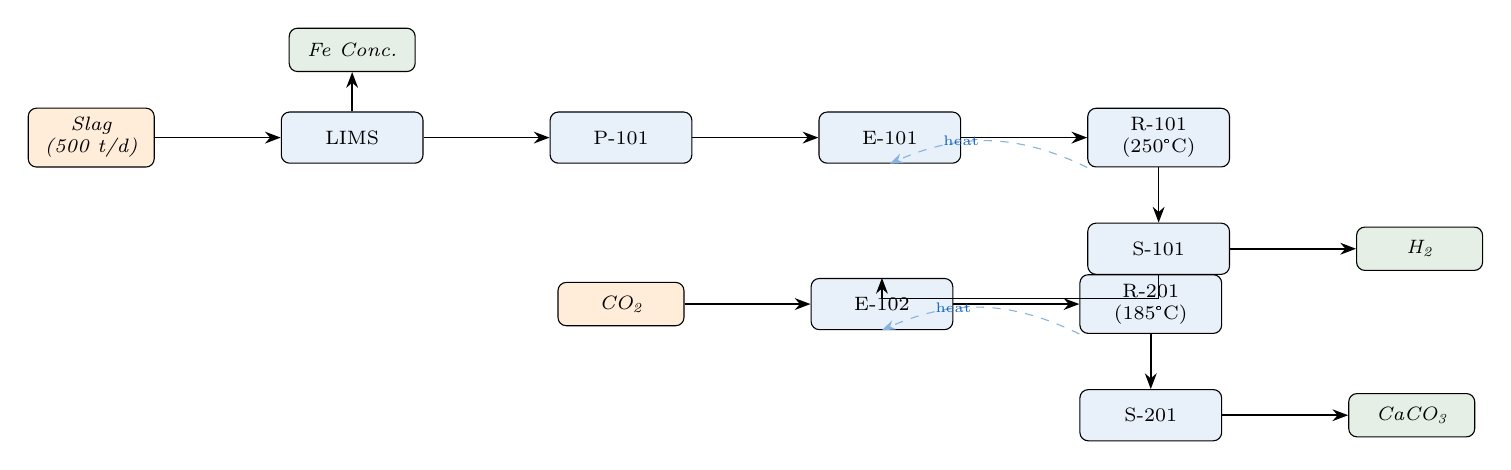
\begin{tikzpicture}[
  node distance=1.0cm and 1.6cm,
  unit/.style={rectangle, draw, rounded corners=3pt, minimum width=1.8cm,
               minimum height=0.65cm, align=center, fill=accent!10, font=\scriptsize},
  product/.style={rectangle, draw, rounded corners=3pt, minimum width=1.6cm,
                  minimum height=0.55cm, align=center, fill=revenue!12,
                  font=\scriptsize\itshape},
  feed/.style={rectangle, draw, rounded corners=3pt, minimum width=1.6cm,
               minimum height=0.55cm, align=center, fill=orange!15,
               font=\scriptsize\itshape},
  stream/.style={-{Stealth[length=2mm]}, semithick},
]

\node[feed] (slag) {Slag\\(500 t/d)};
\node[unit, right=of slag] (lims) {LIMS};
\node[product, above=0.5cm of lims] (fe) {Fe Conc.};
\node[unit, right=of lims] (pump1) {P-101};
\node[unit, right=of pump1] (hx1) {E-101};
\node[unit, right=of hx1] (serp) {R-101\\(250\textdegree C)};
\node[unit, below=0.7cm of serp] (sep) {S-101};
\node[product, right=of sep] (h2) {H\textsubscript{2}};

\node[feed, below=1.5cm of pump1] (co2) {CO\textsubscript{2}};
\node[unit, right=of co2] (hx2) {E-102};
\node[unit, right=of hx2] (carb) {R-201\\(185\textdegree C)};
\node[unit, below=0.7cm of carb] (thick) {S-201};
\node[product, right=of thick] (caco3) {CaCO\textsubscript{3}};

\draw[stream] (slag) -- (lims);
\draw[stream] (lims) -- (fe);
\draw[stream] (lims) -- (pump1);
\draw[stream] (pump1) -- (hx1);
\draw[stream] (hx1) -- (serp);
\draw[stream] (serp) -- (sep);
\draw[stream] (sep) -- (h2);
\draw[stream] (sep.south) -- ++(0,-0.3) -| (hx2);
\draw[stream] (co2) -- (hx2);
\draw[stream] (hx2) -- (carb);
\draw[stream] (carb) -- (thick);
\draw[stream] (thick) -- (caco3);

\draw[-{Stealth}, dashed, accent!50] (serp.south west) to[bend right=25]
    node[left, font=\tiny, accent]{heat} (hx1.south);
\draw[-{Stealth}, dashed, accent!50] (carb.south west) to[bend right=25]
    node[left, font=\tiny, accent]{heat} (hx2.south);

\end{tikzpicture}
\end{center}
\vspace{4pt}
\small
\textbf{Key insight}: Iron removal before carbonation raises pH for carbonate stability (Reaktoro-confirmed).
\end{frame}

% ═══════════════════════════════════════════════════════════════
\begin{frame}{Key Reactions}
\begin{block}{Serpentinization (H\textsubscript{2} Production)}
\vspace{-6pt}
\begin{equation*}
    \text{Fe}_2\text{SiO}_4 + 3\,\text{H}_2\text{O}
    \xrightarrow{250\,^\circ\text{C},\;100\,\text{bar}}
    2\,\text{Fe(OH)}_2 + \text{SiO}_2 + \text{H}_2
\end{equation*}
\end{block}
\vspace{4pt}
\begin{block}{Mineral Carbonation (CO\textsubscript{2} Sequestration)}
\vspace{-6pt}
\begin{align*}
    \text{CaO} + \text{CO}_2 &\xrightarrow{185\,^\circ\text{C},\;50\,\text{bar}} \text{CaCO}_3 \\
    \text{MgO} + \text{CO}_2 &\longrightarrow \text{MgCO}_3
\end{align*}
\end{block}
\end{frame}

% ═══════════════════════════════════════════════════════════════
\section{GDP Analysis}
% ═══════════════════════════════════════════════════════════════

\begin{frame}{Superstructure Overview}
\begin{columns}
\column{0.55\textwidth}
\begin{itemize}
    \item \textbf{15 unit operations} (12 fixed, 3 optional)
    \item \textbf{1 disjunction}: Aux heater \texttt{XOR} Heat recovery only
    \item \textbf{1 optional}: Inter-reactor scrubber
    \item \textbf{4 feasible topologies}
    \item \textbf{12 continuous} design variables for BoTorch
\end{itemize}

\column{0.42\textwidth}
\small
\begin{table}
\centering
\begin{tabular}{@{}cc@{}}
\toprule
\textbf{Heater} & \textbf{Scrubber} \\
\midrule
\checkmark & \checkmark \\
\checkmark & --- \\
--- & \checkmark \\
--- & --- \\
\bottomrule
\end{tabular}
\caption*{4 topologies (2$\times$2)}
\end{table}
\end{columns}
\end{frame}

% ═══════════════════════════════════════════════════════════════
\begin{frame}{Topology Ranking}
\begin{table}
\centering
\small
\begin{tabular}{@{}clccccc@{}}
\toprule
\textbf{Rank} & \textbf{Topology} & \textbf{CAPEX} & \textbf{OPEX}
  & \textbf{EAC} & \textbf{Revenue} & \textbf{Net} \\
& & (\$M) & (\$M/yr) & (\$M/yr) & (\$M/yr) & (\$M/yr) \\
\midrule
\textbf{1} & \textbf{HR only} & \textbf{7.76} & \textbf{2.49} & \textbf{3.28}
  & \textbf{9.53} & \textcolor{revenue}{\textbf{6.25}} \\
2 & HR + scrubber & 7.96 & 2.49 & 3.30 & 9.53 & 6.23 \\
3 & Aux heater & 8.06 & 3.07 & 3.89 & 9.53 & 5.64 \\
4 & Aux + scrub & 8.26 & 3.07 & 3.91 & 9.53 & 5.62 \\
\bottomrule
\end{tabular}
\end{table}
\vspace{6pt}
\centering
\small Aux heater adds \$0.58M/yr OPEX with no measurable benefit.
\end{frame}

% ═══════════════════════════════════════════════════════════════
\section{Results}
% ═══════════════════════════════════════════════════════════════

\begin{frame}{Net Value}
\centering
\vspace{1.5cm}
{\Huge\textbf{\textcolor{revenue}{\$37.87/t}}}\\[14pt]
{\large Net value per tonne of steel slag}\\[12pt]
{\normalsize
\textcolor{revenue}{Revenue: \$57.73/t} \quad
\textcolor{cost}{Cost: \$19.88/t}}\\[6pt]
{\small 500 t/d $\cdot$ 330 d/yr $\cdot$ 20-yr project $\cdot$ 8\% discount}
\end{frame}

% ═══════════════════════════════════════════════════════════════
\begin{frame}{Revenue Breakdown}
\begin{table}
\centering
\begin{tabular}{@{}lrrc@{}}
\toprule
\textbf{Product} & \textbf{Production} & \textbf{Revenue} & \textbf{Share} \\
\midrule
Fe concentrate & 42,075 t/yr & \textcolor{revenue}{\$5.05M/yr} & 53\% \\
CO\textsubscript{2} credits & 58,575 t/yr & \textcolor{revenue}{\$3.51M/yr} & 37\% \\
H\textsubscript{2} gas & 241 t/yr & \textcolor{revenue}{\$0.96M/yr} & 10\% \\
\midrule
\textbf{Total} & & \textcolor{revenue}{\textbf{\$9.53M/yr}} & 100\% \\
\bottomrule
\end{tabular}
\end{table}
\vspace{10pt}
\centering
\small Iron concentrate is the dominant value driver at 53\% of total revenue.
\end{frame}

% ═══════════════════════════════════════════════════════════════
\section{Sensitivity \& Risks}
% ═══════════════════════════════════════════════════════════════

\begin{frame}{Cost Sensitivity (JAX Autodiff)}
\begin{table}
\centering
\begin{tabular}{@{}lrl@{}}
\toprule
\textbf{Parameter} & $|\partial\text{EAC}/\partial x|$ & \textbf{Interpretation} \\
\midrule
Residence time & \$10,185/h & Reactor sizing driver \\
Operating temp & \$8,250/\textdegree C & Energy cost driver \\
Throughput & \$5,214/(t/d) & Economies of scale \\
\bottomrule
\end{tabular}
\end{table}
\vspace{10pt}
\textbf{Key risks:}
\begin{itemize}
    \item CO\textsubscript{2} credits at \$30/t $\to$ net value drops to \$27.22/t
    \item Fe price at \$80/t $\to$ revenue loss of \$1.68M/yr
    \item Serpentinization kinetics require catalyst R\&D
\end{itemize}
\end{frame}

% ═══════════════════════════════════════════════════════════════
\section{Conclusions}
% ═══════════════════════════════════════════════════════════════

\begin{frame}{Key Findings}
\begin{enumerate}
    \item Steel slag valorization at 500 t/d yields \textcolor{revenue}{\textbf{\$37.87/t}} net value
    \item Optimal topology: \textbf{heat recovery only} (no auxiliary heater, no scrubber)
    \item \textbf{Iron concentrate} is the dominant revenue driver (53\%)
    \item \textbf{Iron removal before carbonation} is thermodynamically essential
    \item Aux heater \& scrubber do not justify added cost
\end{enumerate}
\vspace{12pt}
\textbf{Next steps:}
\begin{itemize}
    \item Pilot-scale serpentinization kinetics testing
    \item Detailed vendor quotes for high-pressure reactor vessels
    \item Include Cr/Mn/V value streams (requires expanded thermodynamic database)
\end{itemize}
\end{frame}

\end{document}
